% ----------------------------------------------------------------------------------------------------------
% Eigene Projektbeschreibung und -ergebnisse
% ----------------------------------------------------------------------------------------------------------
\section{Hauptteil - Projektbeschreibung und Projektergebnisse}\label{ergebnisse}
Der Hauptteil soll damit beginnen, die Grundlagen des Lösungsansatzes zu erläutern. Dazu werden zuerst die Mathematischen Grundlagen aufgezeigt. Danach werden die verwendeten selbst erstellten Algorithmen besprochen. Da dabei gewisse Bibliotheken mit Python zum Einsatz kamen, sollen diese im ersten Schritt kurz erwähnt werden. Der finale Software-Aufbau wird vollständig in einem späteren Kapitel vorgestellt.
	
	\subsection{Bibliotheken}
	Der Lasertriangulationssensor wurde vor Allem mit OpenCv und ROS2 entwickelt. OpenCv bietet die perfekte Unterstützung für die benötigte Bildverarbeitung. Diverse Funktionen, um Bilder zu bearbeiten, zur Kamerakalibrierung und zum Errechnen der Ebenengleichung sind in OpenCv implementiert.
	ROS2 kümmert sich um die Automatisierung und den generellen Ablauf eines Scanvorgangs. In der Forschung und Entwicklungs-Projekt mit RINNTECH wird zusätzlich auch ROS2 als übergeordnetes System genutzt. Deshalb war ROS2 auch eine Anforderung an das Projekt. Die vorher benutzte RGB-D-Kamera Intel RealSense ist ebenfalls in der Lage über ROS2 angesprochen zu werden. Da der OpenSource-Lasertriangulationssensor diese ersetzten soll, ist die Verwendung von ROS2 ein logischer Schritt.
	
	\subsection{Der Grundlegende Aufbau}
	Der grundlegende Aufbau orientiert sich an den Lösungsansatz. Notwendig sind dafür nur ein Linienlaser und eine Kamera. Zuerst wurde für einen Prototyp zum Testen eine Webcam verwenden, später eine Industriekamera. Auschlaggebend zum Funktionieren des theoretischen Lösungsansatz ist, dass die Kamera einen Linienversatz aufnehmen kann. Um das zu erreichen werden Kamera und Laser in einem gewissen Winkel zueinander gesetzt. Durch die Perspektive der Kamera entsteht der Linienversatz. Dabei ist egal, ob die Kamera von oben auf das Objekt zeigt und der Laser schräg sitzt oder andersrum. Die Lasertriangulationssensoren aus der Industrie weisen zumeist den Aufbau aus Abb. 1 auf.
	
	\begin{figure}[h]
		\centering
		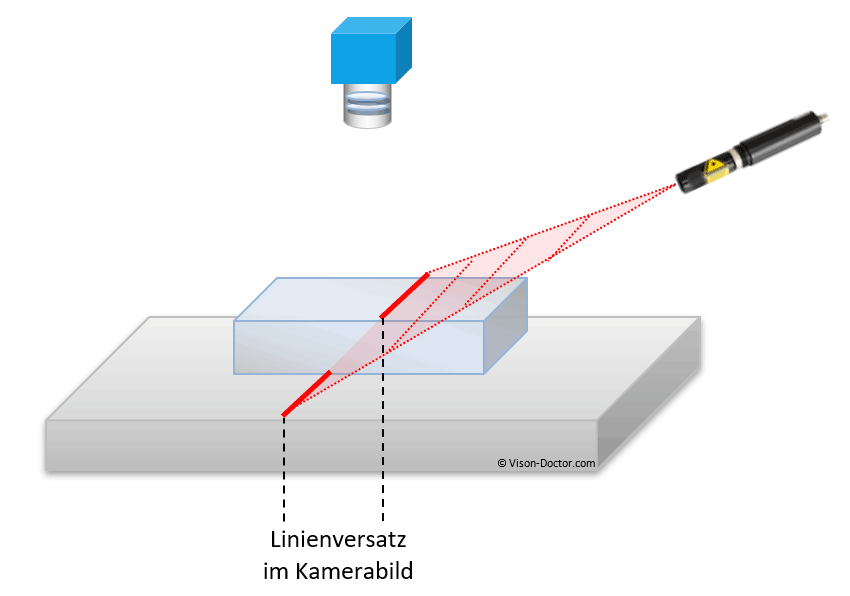
\includegraphics[height=10cm]{img/grundlagen/lasertriangulation_2}
		\caption{Positionen bei der Lasertriangulation}
		\label{lasertriangulation}
	\end{figure}
	
	Der erste Schritt in der Erarbeitung des Sensors war es, die Möglichkeit zu entwickeln, eine aufgenommene Laserlinie in eine korrekte Punktewolke umzusetzen. Danach muss es ermöglicht werden den Sensor über bzw. das Objekt unter dem Sensor bewegen zu können. Mehr zu dem genauen Aufbau des fertigen 3D-Scanner wird im Kapitel 5. Aufbau / Hardware erläutert. Für die folgenden Erklärungen zur mathematischen Grundlage, Bildverarbeitung und Kalibrierung ist nur wichtig zu wissen, dass die Kamera und Laser in einem Winkel zueinander über dem Objekt angebracht sind. 
	
	\subsection{OpenCv Pinhole Camera Model}
	Der Anfang aller Berechnungen des Lasertriangulationssensors ist immer ein Bild. Die Kamera als optischer Sensor ist die einzige Informations-Quelle. Ein Bild besteht aus Pixeln. Diese sind 2-Dimensional. Es muss also eine Möglichkeit gebunden werden, die dritte Dimension zu finden. Für die gesuchten 3D-Punkte des Objektes ist dafür eine Ebenen-Gleichung für die Laser-Ebene notwendig. Diese ist nicht von Anfang an bekannt und es gilt, diese herauszufinden. Trotzdem wird nach einem Vorgehen gesucht, welches nur aus dem Bild und mithilfe der Kamera 3D-Informationen liefern kann. Genau diese Informationen sind zugänglich mit den Pinhole Camera Model von OpenCv. In OpenCv ist eine Kamera genauso, wie eine Lochkamera begriffen.
	
	\begin{figure}[h]
		\centering
		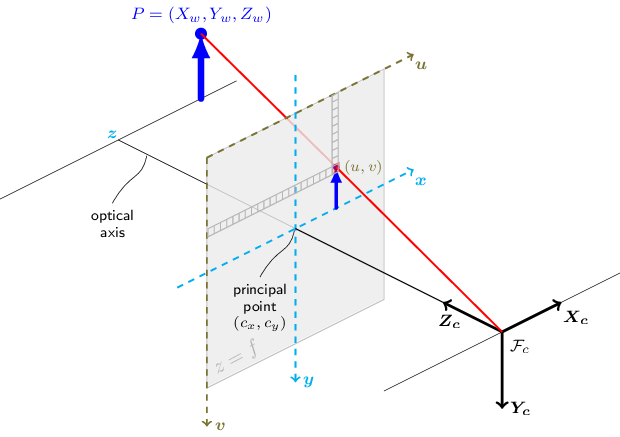
\includegraphics[width=0.7\linewidth]{img/grundlagen/pinhole_camera_model.png}
		\caption[test]{Pinhole Camera Model}
		\captionsource{tesaugdsakif sd}
		\label{fig:pinhole-camera-model}
	\end{figure}

	In Abb. 2 ist dieses Modell dargestellt. Dabei gilt  als optisches Zentrum, welches bei einer Lochkamera das Lochblende ist. Daran orientiert sich das Kamera-Koordinatensystem. Bei einer Lochkamera ist es üblich, dass eine Szene aus der Echten Welt aufgenommen wird. Diese wird über die Öffnung auf dem Kopf gespiegelt auf einem Schirm abgebildet.
	
	
	
	Zum Vergleich ist in Abb. \ref{fig:pinhole-camera-model} das Modell einer Lochkamera zu sehen. Wenn man die beiden Darstellungen vergleicht, fällt auf, dass der „Schirm“, auf dem das Bild als Reflektion dargestellt wird bei der Lochkamera hinter der Lochblende ist und bei dem Modell von OpenCv davor. Die physikalisch korrekte Darstellung ist die der Lochkamera. Jedoch ist OpenCv nicht auf die richtige physikalische Darstellung angewiesen. Mathematisch macht es keinen Unterschied, ob die Bild-Ebene vor oder hinter dem optischen Zentrum ist. So kann ein Punkt in der Szene als Vektor begriffen werden, der durch die Bild-Ebene einen Pixel definiert und zum optischen Zentrum führt. Zu sehen in Abb.2 als die rote Linie. In unserem Fall kennen wir das Bild und die genaue Position eines Pixels mit u und v. Das Ziel ist es 3D-Koordinate zu erhalten.
	
	\subsection{Mathematische Grundlage}
	Grundlegend für die Umrechnung des Pixels in der Bild-Ebene als Vektor mit u und v zu der 3D-Koordinate ist die folgende Formel:
	
	\begin{equation}
		s \; p = A \begin{bmatrix} R|t \end{bmatrix} P_w
		\label{eq:transforamtion}
	\end{equation}
	
	Hierbei ist p der Pixel im Bild. Pw ist die 3D-Koordinate, welche gesucht wird. \( A \) ist die Kamera-Matrix und \( \begin{bmatrix} R|t \end{bmatrix} \) die Rotation und Translation vom Kamera-koordinatensystem zum Weltkoordinatensystem. Kamera-Matrix, Rotation und Translation sind hierbei neu. Die genaue Bedeutung wird in dem Kapitel 4 Kalibrierung genannt. Zum Verstehen der Formel ist hier nur wichtig, dass diese durch eine Kamerakalibrierung herausgefunden werden können. Die Kamera-Matrix und die Rotation sind beides 3x3 Matritzen. Die Translation wird durch einen Vektor beschrieben. In Abbildung 4 wird die Formel noch einmal genauer gezeigt. Aus der Formel sind also p, A und \( \begin{bmatrix} R|t \end{bmatrix} \) bekannt. Unbekannte sind s der Scale-Factor und Pw die Weltkoordinate.
	
		\subsubsection{Homogene Koordinaten}
		In Abbildung 4 sind die Rotation (R), die Translation (t) und die 3D-Weltkoordinate in Homogenen Matrizen bzw. Vektoren dargestellt. Der Vorteil davon ist, dass beliebig viele Transformationen im dreidimensionalen Raum in einer Homogenen Matrix zusammengefasst werden können. Diese kann dann auf einen Punkt im dreidimensionalen Raum, dargestellt als Homogener Vektor, angewandt werden. In diesem Fall sind die Transformationen eine Rotation und eine Translation von dem Punkt im Weltkoordinatensystem zu dem Kamerakoordinatensystem. Es soll kurz die Entstehung der homogenen Matrix für dieses Beispiel erläutert werden.
		
		Die Rotation ist eine 3x3-Matrix:
		
		\( R = \begin{pmatrix} 
		r_{11} & r_{12} & r_{13} \\ r_{21} & r_{22} & r_{23} \\ r_{31} & r_{32} & r_{33} \end{pmatrix} \)
		
		Die Translation ist ein 3x1-Vektor:
		
		\( t = \begin{pmatrix}
		t_1 \\ t_2 \\ t_3
		\end{pmatrix} \)
		
		Die beiden Transformationen wollen wir auf einen Punkt (dargestellt durch den Vektor v) anwenden:
		
		\begin{equation}
			v' = Rv + t
			\label{eq:test}
		\end{equation}
		
		\( v' = Rv + t \)
		
		
		
		Oder ausgeschrieben \ref{eq:test}:
		
		\( v' = \begin{pmatrix}
		r_{11} & r_{12} & r_{13} \\ r_{21} & r_{22} & r_{23} \\ r_{31} & r_{32} & r_{33}
		\end{pmatrix} v + 
		\begin{pmatrix}
		t_1 \\ t_2 \\ t_3
		\end{pmatrix}\)
		
		Eine homogene Matrix ist eine 4x4 -Matrix. Dabei ist die unterste Zeile immer (0, 0, 0, 1). Beide Transformationen können in ihr eingebunden werden:
		
		\( \begin{pmatrix}
		r_{11} & r_{12} & r_{13} & t_1 \\ r_{21} & r_{22} & r_{23} & t_2 \\ 
		r_{31} & r_{32} & r_{33} & t_3 \\ 0 & 0 & 0 & 1
		\end{pmatrix} \)
		
		Diese wird dann mit den 3D-Punkt als homogener Vektor multipliziert:
		
		\( \begin{pmatrix}
		r_{11} & r_{12} & r_{13} & t_1 \\ r_{21} & r_{22} & r_{23} & t_2 \\ 
		r_{31} & r_{32} & r_{33} & t_3 \\ 0 & 0 & 0 & 1
		\end{pmatrix} \times
		\begin{pmatrix}
		v_1 \\ v_2 \\ v_3 \\ 1
		\end{pmatrix} \)
		
		Zur Verdeutlichung:
		
		\( v' =  \begin{pmatrix}
		r_{11} & r_{12} & r_{13} \\ r_{21} & r_{22} & r_{23} \\ r_{31} & r_{32} & r_{33}
		\end{pmatrix} v + 
		\begin{pmatrix}
		t_1 \\ t_2 \\ t_3
		\end{pmatrix} = \begin{pmatrix}
		r_{11} & r_{12} & r_{13} & t_1 \\ r_{21} & r_{22} & r_{23} & t_2 \\ 
		r_{31} & r_{32} & r_{33} & t_3 \\ 0 & 0 & 0 & 1
		\end{pmatrix} \times
		\begin{pmatrix}
		v_1 \\ v_2 \\ v_3 \\ 1
		\end{pmatrix} \)
		
		\subsubsection{Transformationen}
		Die Grundlegende Formel soll jetzt umgestellt werden, um die Variablen zu errechnen, die gebraucht werden. Die angewandten Transformationen werden durch die folgende Abbildung noch einmal verdeutlicht.
		
		Abb. 5: Pinhole Camera Model 2
		
		Das Ziel ist es den 3D-Punkt im Weltkoordinatensystem zu errechnen. Die Rotation (R) und Translation (t) werde für die Umrechnung in das Kamerakoordinatensystem benötigt. Das sind die sogenannten extrinsischen Parameter. Die Kamera-Matrix beschreibt die Transformation zur Bild-Ebene bzw. den Pixel-Koordinaten-System. Die Matrix enthält die sogenannten intrinsischen Parameter. Wir können einen Pixel im Bild auswählen und mithilfe dieser Parameter den entsprechenden Punkt im Weltkoordinatensystem errechnen.
		
		\begin{equation}
			\begin{aligned}
				 \begin{bmatrix} A \end{bmatrix} \begin{bmatrix} R|t \end{bmatrix} p_w &= s \; p_{pix} \\
				 \begin{bmatrix} R|t \end{bmatrix} p_w &= s \begin{bmatrix} A \end{bmatrix}^{-1} p_{pix} \\
				 \begin{bmatrix} R \end{bmatrix} p_w &= s \begin{bmatrix} A \end{bmatrix}^{-1} p_{pix} - t \\
				 p_w &= s \begin{bmatrix} R \end{bmatrix} \begin{bmatrix} A \end{bmatrix}^{-1} p_{pix} - \begin{bmatrix} R \end{bmatrix}^{-1} t
			\end{aligned}
		\end{equation}
		
		Welt zu Kamera:
		
		\begin{equation}
			p_{cam} = \begin{bmatrix} R \end{bmatrix} \; p_w + t
		\end{equation}
		
		Kamera zur Welt:
		
		\begin{equation}
			p_w = \begin{bmatrix} R \end{bmatrix}^{-1} \; (p_{cam} - t)
		\end{equation}
		
	\subsection{Bildverarbeitung}
	
	\subsection{Kalibrierung}
		\subsubsection{Intrinsische}
		\subsubsection{Extrinsische}
		
	\subsection{Aufbau / Hardware}
	
	\subsection{Aufbau / Software}
		\subsubsection{Python (Bibliothek)}
		\subsubsection{ROS2}
		
	\subsection{Qualitative Ergebnisse}
	
	\subsection{Evaluation}
		\subsubsection{Testen von Genauigkeit}
		\subsubsection{Fehler}
		\subsubsection{Probleme und Schwierigkeiten}